\section{Background}

In this work, we explore efficient runtime support for partitioned, global
logical address spaces (PGLAS).  We define the PGLAS data model to be similar
to PGAS data models, which have been in use for over two decades, with the
distinction that data elements are logically addressed using an
application-meaningful {\em key}.  Each key is mapped to a partition of the
global address space and an application can query locality information for a
given key or iterate over local keys, e.g., to support owner-computes models of
work distribution.  In contrast, PGAS models traditionally use a direct
addressing model, such as a remote address (OpenSHMEM and UPC), an offset into
a remote buffer (MPI), or an index into a regular array (Fortran Coarrays).
While there are differences in memory addressing and layout, PGLAS utilizes the
same one-sided, asynchronous data access model as existing PGAS approaches and
data in global space is accessed using one-sided get (read), put
(write), and atomic access functions.  Thus, PGLAS is a member of the broader
family of distributed key/value stores where data organization and access are
similar to PGAS models.

Most PGAS models require global knowledge of data layout in order to
communicate efficiently.  For example, in the OpenSHMEM model, the layout of
the globally accessible space must be identical at all processes.  As a result,
management of globally accessible memory must be performed collectively.  In
contrast, PGLAS introduces a layer of indirection that translates logical
addresses to direct addresses.  The introduction of this layer
has the potential to relax the strong memory management semantics required by
most PGAS models, enabling more dynamic usage models.  In particular, PGLAS can
support dynamic insertions and removals of key/value pairs in the global
address space.

Efficient and scalable support for translation of keys to memory locations is a
performance-critical, new requirement imposed by PGLAS.  Traditional one-sided
communication operations can satisfy the one-sided and asynchronous
requirements of key translation.  However, multiple operations are required to
query a remote translation structure, leading to high overheads~\cite{namashivayam:15}.  We observe
that the user-supplied tag used by MPI runtimes to match an incoming message
(i.e., put) with a posted receive operation supports a key/value-like remote
write model.
%When MPI message processing is performed directly by the NIC,
%this model can be seen to support key/value-style put operations.
However,
there are several key differences between MPI messaging and PGLAS
communication.  First, MPI requires message ordering, whereas PGLAS utilizes
the PGAS unordered-by-default communication model.  Further, when an MPI
runtime receives a message for which there is no matching entry, the message is
treated as unexpected and will be accepted once a matching receive operation is
posted.  In contrast, PGLAS models reject remote accesses to nonexistent keys.
Finally, a posted receive operation is consumed by an incoming message, whereas
a PGLAS model maintains the key/value association until the entry is freed.

% motivation
%\subsection{Hash Tables}
%
%Hash tables are one of the most widely used data
%structures in sequential programs. Data is stored by mapping a key to
%a value. Values may be retrieved in a random access manner by
%providing the key to get or put operations on the hash table.
%%
%% serial vs. parallel approaches
%Hash tables can be implemented with a myriad of different techniques,
%but are traditionally implemented sequentially as an array of pointers
%to objects. Parallel implementations typically distribute table data
%across nodes, requiring that the hash table stores the entire object
%and not simply a reference.
%%
%In this work, we explore the implementation of a parallel, distributed hash
%table as a first implementation of the PGLAS data model.

\subsection{Managing Distributed, Sparse Data}

Of interest to the HPC community, we see PGLAS as a
means for dealing with sparsity. Many common HPC applications rely on
sparse data structures, which causes numerous problems in the hunt for
high performance. Matrix and tensor representations often must contend
with sparse data, resulting in specialized formats such as compressed
sparse row (CSR) and variants. Other problems, such as N-body
simulation, grid and mesh solvers, are naturally expressed using
spatial decomposition trees such as quadtrees and octrees. 

In these cases, there is a natural mapping between an index or
coordinate system and the corresponding data. A global distributed
key/value store could replace a complicated and difficult to parallelize
sparse data structure given the right application.

\subsection{Related Work}

The idea of logically addressing data across memories in a distributed
system has been explored in a number of other models.  Distributed,
shared key/value stores are an intrinsic part of the Piccolo
programming model~\cite{power:10}.  The Linda programming
model~\cite{ahuja:86} is built around tuple spaces, that allows data
to be inserted, read, and removed from global memory. Linda data items
are identified through a user-supplied tuple.  Such models are of
renewed interest in the context of resilience~\cite{wilke:14}.
Distributed object models, such as Orca~\cite{bal:92}, reference
shared data through graphs rather than direct pointers.  In the Open
Community Runtime (OCR)~\cite{OCR}, data blocks (DBs) are identified
by a globally unique ID, which is assigned by the OCR runtime system
and used to portably reference a DB.  Finally, migratable object
models, such as Charm++~\cite{kale:93}, support a variety of methods
for representing and querying object collections.

Hash tables are also commonly used to store sparse or loosely structured
data~\cite{memcached04,chord01,docan:12}
and their implementation has been studied in the context of MPI and popular PGAS
models~\cite{zht13,fompi13,cmpi10,maynard:12,memcached12,mht15} as well as in
the context of RDMA offload~\cite{memcached12,mitchell:13,kalia:14}.  In
addition, PGAS-like hierarchical approaches to
managing sparse spatial decomposition have been proposed~\cite{larkins:08}
along with runtime methods to manage this data and exploit spatial
locality~\cite{larkins:12}.

\section{The Portals Networking Interface}

% portals background

% figure 2.2 / 2.3 in portals spec

%  define NI, PTE
%     - target vs. initiator
%     - wrt SPMD each process plays both roles
%     - define memory descriptor
%     - like a window w MPI?

%  matching interface
%      - define matching, 
%      - ME 
%      -  matching lookup process
%      - priority list

%  define counters and events
%       - define event and counter abstractions
%       - target vs. initiator events / counters
%       - attached to either MD, ME, or PTE
%       - define ct
%            - success vs. failure events
%       - define event
%            - put - target gets put data in event
%            - ack - operation complete
%            - reply - operation completed
%            - flow control


The Portals framework provides several low-level data abstractions that
are used to implement \pdht, our parallel distributed hash table system. \pdht is based on a one-sided
communication model to allow asynchronous data access while avoiding processor
involvement at the target node.  Portals provides support for both
one-sided (a.k.a. non-matching) and matching communication semantics.
Matching communication was designed to support MPI; we describe
a novel application of the Portals matching interface
abstractions to implement a one-sided model that is the basis for
\pdht. By using features in the Portals library,
we can take advantage of network hardware offload~\cite{brightwell:micro:06,bxi} to a greater extent
than if \pdht were implemented using conventional PGAS techniques. Portals defines several concepts
and abstractions that are necessary to the understanding of the
\pdht. The relationship between these different entities is shown in
Figure \ref{fig:portals_put}.

% use figure* to span both cols
\begin{figure}[ht]
  \centering
  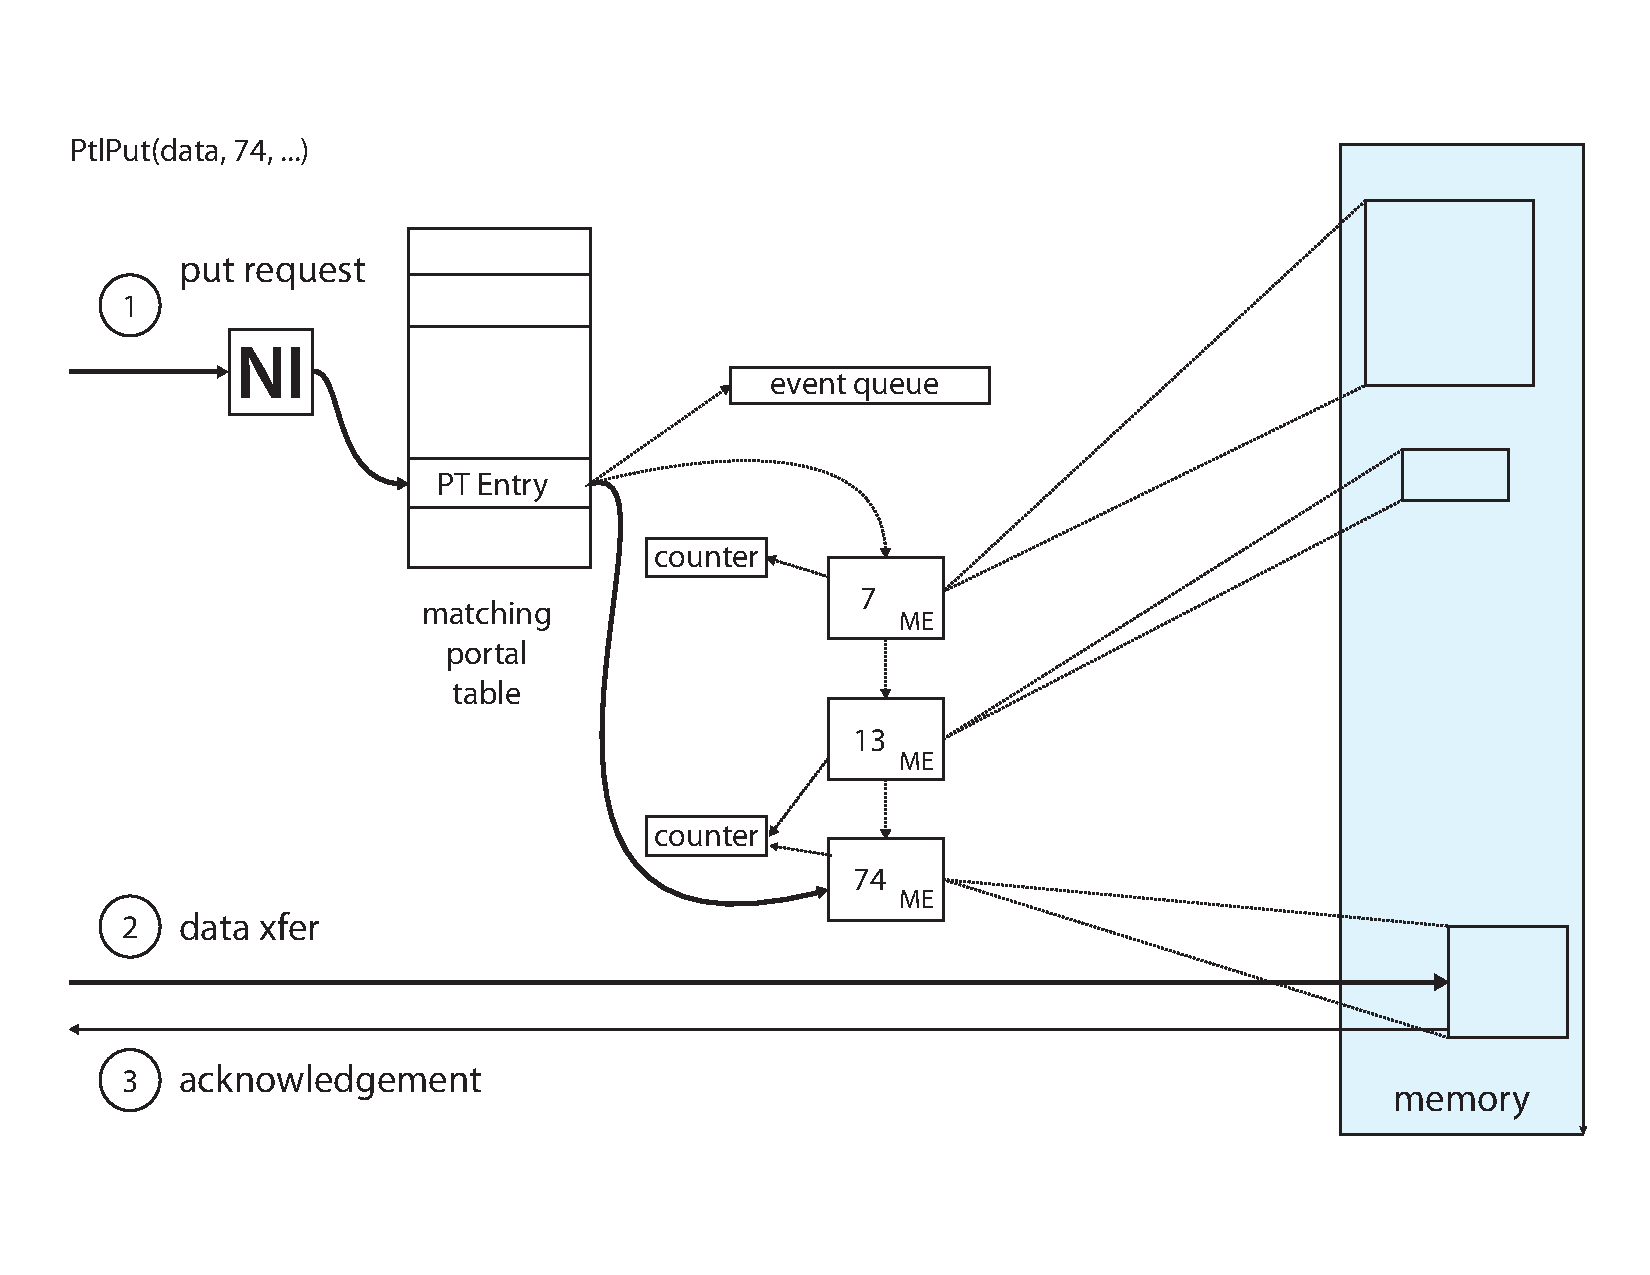
\includegraphics[width=\linewidth]{figs/portals_put}
  \caption{Portals data structures and example put operation using the Portals matching interface.}
  \label{fig:portals_put}
\end{figure}

Portals specifies a {\em network interface} (NI) as a per-process
abstraction of a physical network interface on the target process. The
interface is defined at creation to be either a {\em matching}
or a {\em non-matching} interface, depending on the intended use for
the interface (message-passing or one-sided). \pdht relies on the
Portals matching interface.

Portals defines two primary roles for communication operations. The
{\em initiator} is the process that issues Portals put, get, and atomic operation
requests and the {\em target} is the process receiving
requests. The initiator defines a {\em memory descriptor} (MD), which defines a
region of memory to be used for Portals operations, as well as the
structures used to track communication events for operations utilizing the
given region.  Specific completion information
and notifications may be only visible to the initiator and not the
target, or vice versa.

Target processing is defined in terms of a {\em portal table}. An index into the
portal table is specified on every Portals communication operation and
is used to separate and classify different channels between endpoints.
Every {\em portal table entry} (PTE) maintains a list of memory regions that
are available for communication operations as well as an event queue
to track asynchronous notifications for ongoing communication.

A PTE using the matching interface maintains a list of match-list
entries (ME). Each ME specifies a set of matching criteria and a
memory region associated with the entry. If all of the match criteria
are satisfied, the communication operation commences working on
the corresponding memory region. In particular, each ME contains a 64-bit
{\em match bits} field that must correspond to the match bits
specified on an incoming communication request. For example, a process
would post an {\tt MPI\_Recv()} with a specific match bits
field. Later, Portals would receive a communication request for an
{\tt MPI\_Send()} with the same match bits, which would be correspond
to the posted receive.

Portals provides {\em event queues} and {\em event counters} to track events
relating to initiator- and target-side Portals operations.  Full events contain
detailed information about the event and communication operation involved,
whereas counting events are lighter weight and capture only the success or
failure of a given operation.
Counters are useful for lightweight event counting, where copying a
large amount of data from the Portals implementation to the
application is unnecessary.

On the initiator, an event queue may be associated with an MD, whereas on the
target, a queue may be associated with each PTE.  Counters can also be used to
track both initiator and target events.
Unlike target-side event queues, a counter may be
associated with each ME in the match-list. Multiple MEs may share a
single counter, if desired. \pdht typically uses counters to watch for
successful completion, and full events to track specific failures. More
detailed descriptions of event and counter use within \pdht is
discussed below.

To put everything together, Figure \ref{fig:portals_put} shows the
relationships between the target-side data structures and a sample
{\tt PtlPut()} operation. In this example, we assume that the
initiator process has called {\tt PtlPut} with some data on a matching
interface, with the expected match bits set to 74. When the target
process receives the request, it is dispatched through the
initiator-specified PT index. Next, the match list is searched, until
a 74 is found, or the end of the list is reached. Once the ME has been
located, the {\tt PtlPut} data is copied into the corresponding memory
region. The operation may cause a {\tt PUT} event to be appended to
the event queue or ME success counter to be incremented. An
acknowledgement is sent back to the initiator, possibly generating
another full event or counting event according to the MD that the initiator
supplied to the {\tt PtlPut} operation.



%reply: initiator: remote completion of a get: success = got it, failure = not
%found
%ack: initiator:  put completed
%put: target -> event with put data / ME
%flow control: initiator: disabled NI 

%%% Local Variables:
%%% mode: latex
%%% TeX-master: "paper"
%%% End:
